\begin{ex}%[Mức 2]%[Dự án Giảng 10-11 Nhóm Toán & LaTex, Huỳnh Xuân Tín]%[0D3N1-5]
\immini{Cho hàm số $y=f(x)$ có đồ thị như hình vẽ. Hàm số đã cho đồng biến trên khoảng nào dưới đây?
\choice
{$\left(-\infty;1\right)$}
{$\left(-1;1\right)$}
{$\left(0;1\right)$}
{\True $\left(-1;0\right)$}}
{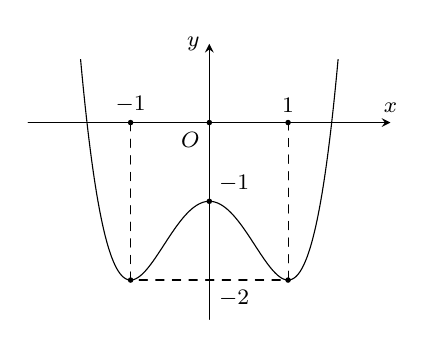
\begin{tikzpicture}[scale=1, font=\footnotesize,line join=round, line cap=round,>=stealth]
\draw[->] (-2.3,0)--(2.3,0) node[above]{$x$};
\draw[->] (0,-2.5)--(0,1) node[left]{$y$};
\draw[dashed] (-1,0)|-(0,-2)-|(1,0);
\begin{scope}
\clip (-2,0.8) rectangle (2,-2.3);
\draw plot[domain=-2:2,smooth,samples=200]
(\x,{(\x)^4-2*(\x)^2-1});
\end{scope}
\fill (0,0) circle(1pt);
\path
(0,0) node[below left]{$O$}
(1,0) node[above]{$1$}
(-1,0) node[above]{$-1$}
(0,-1) node[above right]{$-1$}
(0,-2) node[below right]{$-2$};
\foreach \diemx/\diemy in {-1/0,-1/-2,0/-1,1/-2,1/0}{\fill (\diemx,\diemy)circle(1pt);}
\end{tikzpicture}}
\loigiai{
Từ đồ thị của hàm số $y=f(x)$ suy ra hàm số $y=f(x)$ đồng biến trên khoảng $\left(-1;0\right)$.}
\end{ex}

\begin{ex}%[0D3N1-5]
Trong các hàm số sau, hàm số nào tăng trên khoảng $(-2;0)$?
\choice
{\True $y=x$}
{$y=\dfrac{1}{x}$}
{$y=|x|$}
{$y=x^2$}
\loigiai{Ta có hàm số $y=x$ là hàm số đồng biến trên $\mathbb{R}$ nên hàm số $y=x$ tăng trên $(-2;0)$.}
\end{ex}

\begin{ex}%[Mức 2]Giảng Toán 10, Nguyễn Tài Tuệ]%[0D3N1-5]
Chọn khẳng định đúng?
\choice
{Hàm số $y=f(x)$ được gọi là nghịch biến trên $K$ nếu $\forall x_1 ; x_2 \in K, x_1<x_2 \Rightarrow f\left(x_1\right)<f\left(x_2\right)$}
{Hàm số $y=f(x)$ được gọi là đồng biến trên $K$ nếu $\forall x_1 ; x_2 \in K, x_1<x_2 \Rightarrow f\left(x_1\right) \leq f\left(x_2\right)$}
{Hàm số $y=f(x)$ được gọi là đồng biến trên $K$ nếu $\forall x_1 ; x_2 \in K, x_1<x_2 \Rightarrow f\left(x_1\right)>f\left(x_2\right)$}
{\True Hàm số $y=f(x)$ được gọi là đồng biến trên $K$ nếu $\forall x_1 ; x_2 \in K, x_1<x_2 \Rightarrow f\left(x_1\right)<f\left(x_2\right)$}
\loigiai
{
Hàm số $y=f(x)$ được gọi là đồng biến trên $K$ nếu $\forall x_1 ; x_2 \in K, x_1<x_2 \Rightarrow f\left(x_1\right)<f\left(x_2\right)$
}
\end{ex}

\begin{ex}%[Mức 2]%[Dự án Giảng 10-11 Nhóm Toán & LaTex, Huỳnh Xuân Tín]%[0D3N1-5]
\immini
{Cho hàm số $ y=f(x) $ xác định trên $[-2;2]$, có đồ thị như hình bên. Hàm số đã cho đồng biến trên khoảng nào dưới đây?
\choice
{$(1 ;7)$}
{$(-2;-1)$}
{$(0 ; 1)$}
{\True $(-1 ; 0)$}
}
{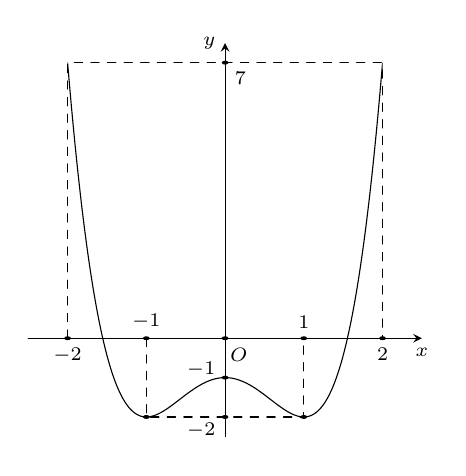
\begin{tikzpicture}[yscale=0.5, font=\footnotesize, line join=round, line cap=round, >=stealth]
\def\a{1}
\def\b{-2}
\def\c{-1}
\draw[dashed](-1,0)node[above]{\scriptsize$ -1 $}|-(0,-2)-|(1,0)node[above]{\scriptsize$ 1 $}(0,-1)node[left,yshift=3pt]{\scriptsize$ -1 $}(0,-2)node[left,yshift=-5pt]{\scriptsize$ -2 $};
\draw[->] (-2.5,0) -- (2.5,0) node[below] {\scriptsize $x$};
\draw[->] (0,-2.5) -- (0,7.5) node[left] {\scriptsize $y$};
\draw (0,0)node[below,xshift=5pt]{\scriptsize $O$};
\foreach \x/\y in {-1/0,0/0,1/0,-1/-2,1/-2,0/-1,0/-2,0/7,-2/0,2/0} \draw[fill=black] (\x,\y) circle (1pt);
\draw[dashed] (-2,0)node[below]{\scriptsize$-2$}--(-2,7)--(2,7)--(2,0)node[below]{\scriptsize$2$};
\clip (-2,-2.1)rectangle(2,7.5);
\draw[samples=150,smooth,domain=-2:2] plot(\x,{\a*(\x)^4+(\b)*(\x)^2+(\c)});
\draw (0,7)	node[below right]{\scriptsize$7$};
\end{tikzpicture}}
\loigiai{
Từ đồ thị của hàm số đã cho ta suy ra hàm số đã cho đồng biến trên khoảng $ \left(-1;0\right)  $ và $ \left(1;2\right)  $.}
\end{ex}

\begin{ex}%[Mức 1]%[N]giảng 10 New - 4in1, Nguyễn Vân Trường]%[0D3N1-5]
Cho hàm số $y=x^2-2x+3$.
\choice
{Hàm số nghịch biến trên khoảng $\left( 1;+\infty\right) $}
{\True Hàm số nghịch biến trên khoảng $\left( -\infty;1\right) $}
{Hàm số đồng biến trên $\mathbb{R}$}
{Hàm số đồng biến trên khoảng $\left( -\infty;1\right) $}
\loigiai{
Hàm số bậc hai với $a=1>0$ và $-\dfrac{b}{2a}=1$ có bảng biến thiên:
\begin{center}

\begin{tikzpicture}[scale=1.2,>=stealth]
\tkzTabInit[nocadre=false,lgt=1,espcl=2,deltacl=0.5]{$x$/.7,$y$/2}
{$-\infty$ , $1$ , $+\infty$}
\tkzTabVar{+/$+\infty$ , -/$2$ , +/$+\infty$}
\end{tikzpicture}
\end{center}
Vậy hàm số nghịch biến trên khoảng $\left( -\infty;1\right)$ .
}
\end{ex}

\begin{ex}%[0D3N2-3]
Parabol $(P)\colon y=x^2-4 x+5$ có phương trình trục đối xứng là
\choice
{$x=-1$}
{$x=-2$}
{$x=1$}
{\True $x=2$}
\loigiai{
Phương trình trục đối xứng của $y=x^2-4x+5$ là $x=-\dfrac{-4}{2\cdot 1}\Leftrightarrow x=2$.
}
\end{ex}

\begin{ex}%[0D3N2-3]
Trục đối xứng của parabol $y=-x^2+5x+3$ là đường thẳng có phương trình
\choice
{$x=\dfrac{5}{4}$}
{$x=-\dfrac{5}{2}$}
{$x=-\dfrac{5}{4}$}
{\True $x=\dfrac{5}{2}$}
\loigiai{
Trục đối xứng $x=-\dfrac{b}{2a}=\dfrac{5}{2}$.
}
\end{ex}

\begin{ex}%[Dự án EX-10-11-Chuẩn hóa]%[Hoàng Thanh Phương]%[0D3N2-3]
Cho hàm số $y=2x^2-x+3$, điểm nào thuộc đồ thị hàm số?
\choice{\True $M(0;3)$}{$M(2;3)$}{$M(-1;1)$}{$M(2;1)$}
\loigiai{
Điểm $M(0;3)$ thuộc đồ thị hàm số trên.
}
\end{ex}

\begin{ex}%[0D3N2-3]
Đồ thị của hàm số $y=a{x^2}+x+a$ đi qua điểm $A(1;2)$. Giá trị của $a$ là
\choice
{$a=\dfrac{2}{3}$}
{$a=-\dfrac{2}{3}$}
{$a=-\dfrac{1}{2}$}
{\True $a=\dfrac{1}{2}$}
\loigiai{
Đồ thị của hàm số $y=a{x^2}+x+a$ đi qua điểm $A(1;2)\Leftrightarrow a+1+a=2\Leftrightarrow a=\dfrac{1}{2}$.}
\end{ex}

\begin{ex}%[0D3N2-3]

Cho hàm số $y=f\left( x \right)=a{x^2}+bx+c$ có đồ thị hàm số như hình vẽ. Đặt $\Delta =b^2-4ac$, tìm dấu của $a$ và $\Delta $ ?\\
\begin{center}
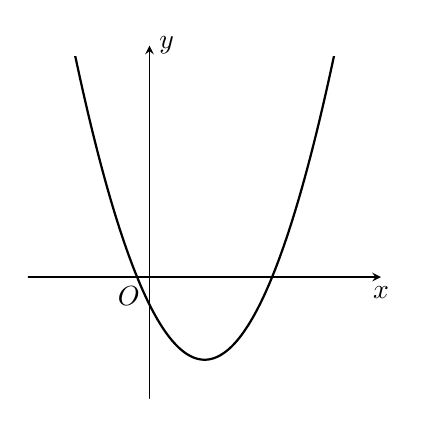
\begin{tikzpicture}[scale=0.7, line join=round, line cap=round, >=stealth]
\tikzset{every node/.style={scale=1}}
\def\xmin{-2}\def\xmax{4}\def\ymin{-2}\def\ymax{4}
\draw[->] (\xmin-0.2,0)--(\xmax+0.2,0) node[below]{$x$};
\draw[->] (0,\ymin-0.2)--(0,\ymax+0.2) node[right]{$y$};
\draw (0,0) node[below left]{$O$};
\foreach \x in {}\draw (\x,0.1)--(\x,-0.1) node[below]{$\x$};
\foreach \y in {}\draw (0.1,\y)--(-0.1,\y) node[left]{$\y$};
\clip (\xmin,\ymin) rectangle (\xmax,\ymax);
\draw[thick,smooth,samples=200,domain=\xmin:\xmax] plot (\x,{1*((\x)^2)-2*\x-1/2});
\end{tikzpicture}
\end{center}
\choice
{\True $a>0;\Delta >0$}
{ $a<0;\Delta >0$}
{ $a<0;\Delta =0$}
{ $a>0;\Delta <0$}
\loigiai{
\begin{itemize}
\item Đồ thị hàm số $y=f\left( x \right)=a{x^2}+bx+c$ có bề lõm quay lên trên nên $a>0$.
\item Đồ thị hàm số $y=f\left( x \right)=a{x^2}+bx+c$ cắt trục hoành tại hai điểm phân biệt nên $\Delta >0$.
\end{itemize}
}
\end{ex}

\begin{ex}%[0D3H2-3]
Đồ thị hàm số $y=a{x^2}+bx+c\,(a>0)$ có điểm thấp nhất là
\choice
{\True $I\left(-\dfrac{b}{2a};-\dfrac{\Delta}{4a}\right)$}
{$I\left(-\dfrac{b}{a};-\dfrac{\Delta}{4a}\right)$}
{$I\left(\dfrac{b}{2a};\dfrac{\Delta}{4a}\right)$}
{$I\left(-\dfrac{b}{2a};\dfrac{\Delta}{4a}\right)$}
\loigiai{
Đồ thị hàm số $y=a{x^2}+bx+c\,(a>0)$ có điểm thấp nhất là đỉnh của parabol $I\left(-\dfrac{b}{2a};-\dfrac{\Delta}{4a}\right)$.}
\end{ex}

\begin{ex}%[0-HK1-CD-7-DaPhuc-HaNoi-2324]%[VN-MT-6,Trần Thị Hồng]%[0D3H2-3]
Tọa độ đỉnh của parabol $(P)\colon y=2x^2-4x$ là
\choice
{$I(0;2)$}
{$I(2;0)$}
{\True$I(1;-2)$}
{$I(-2;1)$}
\loigiai{ Ta có $-\dfrac{b}{2a}= 1$ và $-\dfrac{\Delta}{4a}=-2$. Do đó tọa độ đỉnh của $(P)$ là $I(1;-2)$.}
\end{ex}

\begin{ex}%[0D3H2-3]
\immini{
Đồ thị hình bên dưới là đồ thị của hàm số bậc hai nào?
\choice
{$y=x^2-3x+1$}
{\True $y=2x^2-3x+1$}
{$y=-x^2+1$}
{$y=-2x^2+x+1$}
}
{
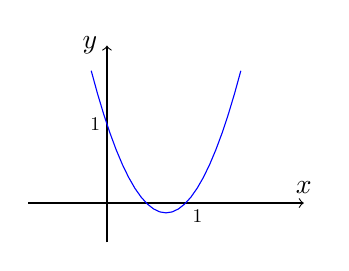
\begin{tikzpicture}
\draw[->] (-1,0)--(2.5,0)node[above]{$x$}; % Hệ trục tọa độ
\draw[->] (0,-.5)--(0,2)node[left]{$y$};
\draw [domain=-0.2:1.7, blue] plot (\x, {2*(\x)^2-3*(\x)+1});
\fill[black] (1,0)node[below right, scale=.7]{$1$}
(0,1)node[left, scale=.7]{$1$};
\end{tikzpicture}
}
\loigiai{
Từ đồ thị $\Rightarrow a>0$, điểm $M(1; 0)\in (P)$ nên hàm số đúng là $y=2x^2-3x+1$.
}
\end{ex}

\begin{ex}%[0D3H2-3]
Tọa độ đỉnh của đồ thị hàm số của parabol có phương trình $y=-x^2+2x+3$ là
\choice
{$(-1;0)$}
{$(2;3)$}
{\True $(1;4)$}
{$(1;0)$}
\loigiai{
Ta có parabol $P \colon y=-x^2+2x+3$.
Tọa độ đỉnh $\left(-\dfrac{b}{2a}; f\left(-\dfrac{b}{2a}\right)\right) = (1;4)$.
}
\end{ex}

\begin{ex}%[HK1, SoBacNinh, 2023-2024]%[0D3H2-3]
\immini{
Cho hàm số bậc hai $y=ax^2+bx+c\,(a,b,c\in\mathbb{R})$ có đồ thị như hình vẽ bên. Mệnh đề nào sau đây đúng?
\choice
{$a>0,\,b>0,\,c>0$}
{\True $a<0,\,b<0,\,c>0$}
{$a>0,\,b<0,\,c>0$}
{$a<0,\,b<0,\,c<0$}
}{
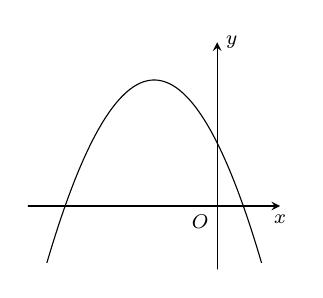
\begin{tikzpicture}[scale=0.8, font=\footnotesize, line join=round, line cap=round, >=stealth]
\tikzset{every node/.style={scale=0.9}}
\draw[->] (-3,0)--(1,0) node[below] {$x$};
\draw[->] (0,-1)--(0,2.6) node[right] {$y$};
\draw (0,0) node [below left] {$O$};
\begin{scope}
\clip (-3,-0.9) rectangle (1.1,2.7);
\draw[samples=200,domain=-3.3:0.8,smooth,variable=\x] plot (\x,{-1*(\x+1)^2+2});
\end{scope}
\end{tikzpicture}
}
\loigiai{
Parabol có bề lõm quay xuống dưới nên $a<0$.\\
Parabol giao với trục tung tại điểm có tung độ dương nên $c>0$.\\
Parabol có trục đối xứng nằm bên trái trục tung nên $-\dfrac{b}{2a}<0\Rightarrow b<0$ (do $a<0$).\\
Vậy $a<0,\,b<0,\,c>0$.
}
\end{ex}

\begin{ex}%[0D7N1-1]%[Dự án đề kiểm tra Toán 10 HKII NH23-24-TrungKien]%[THPT TranHungDao-TPHCM]
Biểu thức nào sau đây {\bf không} là tam thức bậc hai?
\choice
{$f(x)=2x^2-5x+1$}
{$f(x)=-3x^2-8x$}
{\True $f(x)=x^4-3x^2+1$}
{$f(x)=(x-1)(1-3x)$}
\loigiai{
Biểu thức $f(x)=x^4-3x^2+1$ không là một tam thức bậc hai.
}
\end{ex}

\begin{ex}%[0D7N1-1]
Trong các biểu thức sau, biểu thức nào là tam thức bậc hai?
\choice
{\True $f(x)=x^2+3$}
{$f(x)=2 x+3$}
{$f(x)=mx^2+3$}
{$f(x)=\sqrt{2 x^2+3}$}
\loigiai{
Theo định nghĩa, tam thức bậc hai là $f(x)=x^2+3$.
}
\end{ex}

\begin{ex}%[0D7N1-1]
Biểu thức nào sau đây là một tam thức bậc hai đối với $x$?
\choice
{\True $f(x)=4x^2-\sqrt{7}$}
{$f(x)=2x-8$}
{$f(x)=\dfrac{x^2-1}{2x}$}
{$f(x)=\dfrac{x^2-x+1}{x+2}$}
\loigiai{
Biểu thức là một tam thức bậc hai đối với $x$ là $f(x)=4x^2-\sqrt{7}$.
}
\end{ex}

\begin{ex}%[0D7N1-1]
Cho $f(x)=ax^2+bx+c$ ($a\neq 0$). Điều kiện để $f(x)>0$, $\forall x \in \mathbb{R}$ là
\choice
{ $\heva{&a>0 \\& \Delta \leq 0}$}
{ $\heva{&a>0 \\& \Delta \geq 0}$}
{\True $\heva{&a>0 \\& \Delta<0}$}
{ $\heva{&a<0 \\& \Delta>0}$}
\loigiai{
Ta có đáp án cần tìm là $\heva{&a>0 \\& \Delta<0}$.
}
\end{ex}

\begin{ex}%[De-chuan-hoa-so-8]%[Duong Xuan Loi]%[0D7N1-2]
Cho tam thức bậc hai $f(x)=ax^2+bx+c$, $(a \neq 0)$. Điều kiện cần và đủ để $f(x) \le 0, \forall x \in \mathbb{R}$ là
\choice
{$\heva{& a<0 \\ & \Delta>0}$}
{$\heva{& a<0 \\ & \Delta>0}$}
{$\heva{& a>0 \\ & \Delta \geq 0}$}
{\True $\heva{& a<0 \\ & \Delta \leq 0}$}
\loigiai{
Tam thức bậc hai $f(x)=a x^2+bx+c$, $(a \neq 0)$ luôn cùng dấu với $a$ khi $\Delta<0$.\\
Do đó điều kiện cần và đủ để $f(x) \le 0, \forall x \in \mathbb{R}$ là $\heva{& a<0 \\ & \Delta \le 0.}$
}
\end{ex}

\begin{ex}%[Dự án Đề GK2 PNL Cấu Trúc 2025]%[Đào-V- Thuỷ]%[0D7N1-2]
Cho tam thức bậc hai $f(x)= ax^2+bx+c$ ($a\neq 0$). Điều kiện để $f(x) \le 0$, $\forall x\in \mathbb{R}$ là
\def\dotEX{}
\choice
{$\heva{&a>0\\ &\Delta\le 0.}$}
{\True $\heva{&a<0\\ &\Delta \le 0.}$}
{$\heva{&a>0\\ &\Delta\ge 0.}$}
{$\heva{&a<0\\ &\Delta\ge 0.}$}
\loigiai
{
Điều kiện để $f(x) \le 0$, $\forall x\in \mathbb{R}$ là $\heva{&a<0\\ &\Delta \le 0.}$
}
\end{ex}

\begin{ex}%[0D7N1-2]%[tex hóa đề CK2 - 2025 - Huyên Nguyễn]
Tập nghiệm của phương trình
$\sqrt{x^2-x+1}=\sqrt{x^2+2x+4}$ là
\choice
{ $\mathrm{S} = \{1\}$}
{\True$\mathrm{S} = \{-1\}$}
{$\mathrm{S} = \{0\}$}
{$\mathrm{S} = \varnothing$}
\loigiai{
Ta có \begin{eqnarray*}
\sqrt{x^2-x+1}=\sqrt{x^2+2x+4}&\Leftrightarrow& x^2-x+1=x^2+2x+4\\
&\Leftrightarrow& 3x=-3\\
&\Leftrightarrow& x=-1.
\end{eqnarray*}
Vậy $\mathrm{S} = \{-1\}$.
}
\end{ex}

\begin{ex}%[0D7N1-2]
Cho $f(x)=a x^2+b x+c$ $(a \ne 0)$. Điều kiện để $f(x)>0$, $\forall x \in \mathbb{R}$ là
\choice
{$\heva{&a>0\\& \Delta \le 0}$}
{$\heva{&a>0\\& \Delta \ge 0}$}
{\True $\heva{&a>0\\& \Delta < 0}$}
{$\heva{&a<0\\& \Delta > 0}$}
\loigiai{ Điều kiện để $f(x)>0$, $\forall x \in \mathbb{R}$ là $\heva{&a>0\\& \Delta < 0.}$}
\end{ex}

\begin{ex}%[10-11-12EX-GHK2-2425]%[Dương Quang]%[0D7N1-2]
\lq\lq Cho tam thức bậc hai $f(x)=ax^2+bx+c$ ($a\neq0$). Nếu $\Delta>0$ và $x_1$, $x_2$ là hai nghiệm của $f(x)$ ($x_1<x_2$) thì $f(x)$ ...(1)... với $a$ với mọi $x$ thuộc khoảng $(x_1;x_2)$; $f(x)$ ...(2)... với $a$ với mọi $x$ thuộc hai khoảng $(-\infty;x_1)$, $(x_2;+\infty)$\rq\rq. Nội dung đúng trong các ô trống (1), (2) lần lượt là
\choice
{trái dấu, trái dấu}
{cùng dấu, trái dấu}
{cùng dấu, cùng dấu}
{\True trái dấu, cùng dấu}
\loigiai{
Cho tam thức bậc hai $f(x)=ax^2+bx+c$ ($a\neq0$).\\
Nếu $\Delta>0$ và $x_1$, $x_2$ là hai nghiệm của $f(x)$ ($x_1<x_2$) thì $f(x)$ trái dấu với $a$ với mọi $x$ thuộc khoảng $(x_1;x_2)$; $f(x)$ cùng dấu với $a$ với mọi $x$ thuộc hai khoảng $(-\infty;x_1)$, $(x_2;+\infty)$.
}
\end{ex}

\begin{ex}%[0H5N2-1]%[KNTT - Lớp 10 - Ôn tập cuối học kì 1 - Đề 6]%[Nguyễn Hoài Nam]
Cho $3$ điểm phân biệt $A$, $B$, $C$. Trong các khẳng định sau, khẳng định nào \textbf{sai}?
\choice
{$\overrightarrow{CA}-\overrightarrow{CB}=\overrightarrow{AB}$}
{$\overrightarrow{AC}+\overrightarrow{CB}=\overrightarrow{AB}$}
{$\overrightarrow{CA}+\overrightarrow{BC}=\overrightarrow{BA}$}
{\True $\overrightarrow{CB}-\overrightarrow{AC}=\overrightarrow{BA}$}
\loigiai{
Khẳng định 	$\overrightarrow{CB}+\overrightarrow{AC}=\overrightarrow{BA}$ sai vì 	$\overrightarrow{CB}+\overrightarrow{AC}=\overrightarrow{AB}$.}
\end{ex}

\begin{ex}%[Đề ôn tập số 02-Tổng hiệu hai véc-tơ]%[Nguyễn Trung Kiên, dự án BG10]%[0H5N2-1]
Gọi $M$ là trung điểm của đoạn thẳng $AB$. Khẳng định nào sau đây là \textbf{sai}?
\choice
{Hai véc-tơ $\overrightarrow{MA}$ và $\overrightarrow{MB}$ ngược hướng}
{$\overrightarrow{AM}=-\overrightarrow{BM}$}
{\True $\overrightarrow{MA}=\overrightarrow{MB}$}
{$\overrightarrow{MA}+\overrightarrow{MB}=\overrightarrow{0}$}
\loigiai
{
\begin{center}
\begin{tikzpicture}[font=\footnotesize, line join=round, line cap=round, >=stealth, scale=1]
\draw (0,0) coordinate(A) -- (6,0) coordinate(B)
($(A)!1/2!(B)$) coordinate(M);
\foreach \i in {A,B,M} \fill (\i) node[below]{$\i$} circle(1pt);
\end{tikzpicture}
\end{center}
Ta có $\overrightarrow{MA}$, $\overrightarrow{MB}$ là hai véc-tơ đối nhau nên $\overrightarrow{MA}=-\overrightarrow{MB}$.}
\end{ex}

\begin{ex}%[De-chuan-hoa-so-11]%[Đoàn Hùng]%[0H5N2-1]
Véc-tơ tổng $\overrightarrow{M N}+\overrightarrow{P Q}+\overrightarrow{N P}+\overrightarrow{Q R}$ bằng
\choice
{\True $\overrightarrow{MR}$}
{$\overrightarrow{MN}$}
{$\overrightarrow{PR}$}
{$\overrightarrow{MP}$}
\loigiai{
Ta có $\overrightarrow{M N}+\overrightarrow{P Q}+\overrightarrow{N P}+\overrightarrow{Q R}=\overrightarrow{M N}+\overrightarrow{N P}+\overrightarrow{P Q}+\overrightarrow{Q R}=\overrightarrow{MR}$.
}
\end{ex}

\begin{ex}%[0-TK-HK1-CT-2-2425]%[VN-MT-9-CT-10-11, Võ Nguyên Thạch]%[0H5N2-1]
Cho ba điểm $A$, $B$, $C$ bất kỳ. Khẳng định nào sau đây \textbf{đúng}?
\choice
{\True $\overrightarrow{AB}+\overrightarrow{BC}=\overrightarrow{AC}$}
{$\overrightarrow{BA}+\overrightarrow{BC}=\overrightarrow{AC}$}
{$\overrightarrow{AB}-\overrightarrow{AC}=\overrightarrow{BC}$}
{$\overrightarrow{CA}+\overrightarrow{BA}=\overrightarrow{CB}$}
\loigiai{
Theo quy tắc ba điểm ta có $\overrightarrow{AB}+\overrightarrow{BC}=\overrightarrow{AC}$.
}
\end{ex}

\begin{ex}%[Dự án giảng K10-11, Phan Văn Thành]%[0H5N2-1]
Cho tam giác $ABC$, trọng tâm $G$. Kết luận nào sau đây đúng?
\choice
{Không xác định được $\overrightarrow{GA}+\overrightarrow{GB}+\overrightarrow{GC}$}
{$\overrightarrow{GA}=\overrightarrow{GB}=\overrightarrow{GC}$}
{\True $\overrightarrow{GA}+\overrightarrow{GB}+\overrightarrow{GC}=\overrightarrow{0}$}
{$\overrightarrow{GC}=\overrightarrow{GA}+\overrightarrow{GB}$}
\loigiai{
Theo quy tắc trọng tâm của tam giác thì $\overrightarrow{GA}+\overrightarrow{GB}+\overrightarrow{GC}=\overrightarrow{0}$.
}
\end{ex}

\begin{ex}%[0H5N2-1]
Cho tứ diện $ABCD$. Lấy $G$ là trọng tâm của tam giác $ABC$. Phát biểu nào sau đây là \textbf{sai}?
\choice
{$\overrightarrow{GA}+\overrightarrow{GB}+\overrightarrow{GC}=\overrightarrow{0}$}
{\True $\overrightarrow{GA}+\overrightarrow{GB}+\overrightarrow{GC}+\overrightarrow{GD}=\overrightarrow{0}$}
{$\overrightarrow{GD}-\overrightarrow{GA}=\overrightarrow{AD}$}
{$\overrightarrow{DA}+\overrightarrow{DB}+\overrightarrow{DC}=3\overrightarrow{DG}$}
\loigiai{ Ta có
\begin{itemize}
\item $\overrightarrow{GA}+\overrightarrow{GB}+\overrightarrow{GC}=\overrightarrow{0}$ đúng, vì $G$ là trọng tâm tam giác $ABC$.
\item Ta có
\begin{eqnarray*}
&&\overrightarrow{GA}+\overrightarrow{GB}+\overrightarrow{GC}+\overrightarrow{GD}=\overrightarrow{0}\\
&\Leftrightarrow&\overrightarrow{0}+\overrightarrow{GD}=\overrightarrow{0}\\
&\Leftrightarrow&\overrightarrow{GD}=\overrightarrow{0} \text{(sai)}.
\end{eqnarray*}
\item $\overrightarrow{GD}-\overrightarrow{GA}=\overrightarrow{AD}$ đúng.
\item Ta có
\begin{eqnarray*}
&&\overrightarrow{DA}+\overrightarrow{DB}+\overrightarrow{DC}=3\overrightarrow{DG}\\
&\Leftrightarrow&	\overrightarrow{DG}+\overrightarrow{GA}+\overrightarrow{DG}+\overrightarrow{GB}+\overrightarrow{DG}+\overrightarrow{GC}=3\overrightarrow{DG}\\
&\Leftrightarrow&	3\overrightarrow{DG}+\overrightarrow{GA}+\overrightarrow{GB}+\overrightarrow{GC}=3\overrightarrow{DG}\\
&\Leftrightarrow&	3\overrightarrow{DG}+\overrightarrow{0}=3\overrightarrow{DG} \text{ (đúng)}.
\end{eqnarray*}
\end{itemize}

}
\end{ex}

\begin{ex}%[0H5N2-1]%[CTST - Lớp 10 - Ôn tập cuối học kì 1 - Đề 2]%[Cao Thành Thái]
Cho ba điểm $M$, $N$, $P$. Véc-tơ $\overrightarrow{u} = \overrightarrow{NP} + \overrightarrow{MN}$ bằng véc-tơ nào dưới đây?
\choice
{$\overrightarrow{PN}$}
{$\overrightarrow{PM}$}
{\True $\overrightarrow{MP}$}
{$\overrightarrow{NM}$}
\loigiai
{
Ta có $\overrightarrow{u} = \overrightarrow{NP} + \overrightarrow{MN} = \overrightarrow{MN} + \overrightarrow{NP} = \overrightarrow{MP}$.
}
\end{ex}

\begin{ex}%[Dự án Form mới 12/4/6-HK1 Lớp 10-11]%[VN-MT-6, Võ NGuyên Thạch]%[THPT TÂN TÚC-TP HCM]%[0H5N2-1]
Cho tam giác $ABC$ có trọng tâm $G$, tổng ba vectơ $\overrightarrow{GA}+\overrightarrow{GB}+\overrightarrow{GC}$ bằng
\choice
{\True $\overrightarrow{0}$}
{$\overrightarrow{AC}$}
{$\overrightarrow{CB}$}
{$\overrightarrow{BC}$}
\loigiai{
Với $G$ là trọng tâm tam giác $ABC$ ta có $\overrightarrow{GA}+\overrightarrow{GB}+\overrightarrow{GC}=\overrightarrow{0}$.
}
\end{ex}

\begin{ex}%[Dự án giảng K10-11, Phan Văn Thành]%[0H5N2-1]
Cho bốn điểm bất kỳ $A,B,C,O$. Mệnh đề nào sau đây là đúng?
\choice
{$\overrightarrow{OA}=\overrightarrow{OB}-\overrightarrow{BA}$}
{$\overrightarrow{OA}=\overrightarrow{CA}+\overrightarrow{CO}$}
{\True $\overrightarrow{BC}-\overrightarrow{AC}+\overrightarrow{AB}=\overrightarrow{0}$}
{$\overrightarrow{BA}=\overrightarrow{OB}-\overrightarrow{OA}$}
\loigiai{
Ta có $\overrightarrow{BC}-\overrightarrow{AC}+\overrightarrow{AB}=\overrightarrow{AB}+\overrightarrow{BC}-\overrightarrow{AC}=\overrightarrow{AC}-\overrightarrow{AC}=\overrightarrow{0}$.
}
\end{ex}

\begin{ex}%[0-HK1-KN-8-TranHungDao-HaNoi-2324]%[VN-MT-6,Nguyễn Kiều Nhã Tú]%[0H5N2-1]
Cho ba điểm $A$, $B$, $C$. Vectơ $\overrightarrow{v}=\overrightarrow{AC}-\overrightarrow{AB}$ bằng vectơ nào sau đây?
\choice
{$\overrightarrow{AC}$}
{$\overrightarrow{CB}$}
{\True $\overrightarrow{BC}$}
{$\overrightarrow{AB}$}
\loigiai{
Ta có $\overrightarrow{v}=\overrightarrow{AC}-\overrightarrow{AB}=\overrightarrow{BA}+\overrightarrow{AC}=\overrightarrow{BC}$.
}
\end{ex}

\begin{ex}%[0-HK1-CT-6-HungVuong-HCM-2324]%[VN-MT-6, Nguyễn Hữu Đức]%[0D3V2-6]
\immini[thm]{Một bức tường hình dạng một parabol $(P)$ có trục đối xứng là $SO$ (như hình vẽ). Biết chiều cao $SO=8$\,m, bề rộng chân tường $AB=10$\,m. Người ta muốn treo một bức tranh để trang trí có dạng hình chữ nhật $MNPQ$ với $O$ là trung điểm của cạnh $MN$ và $MN=5$\,m. Tính diện tích bức tranh.
}
{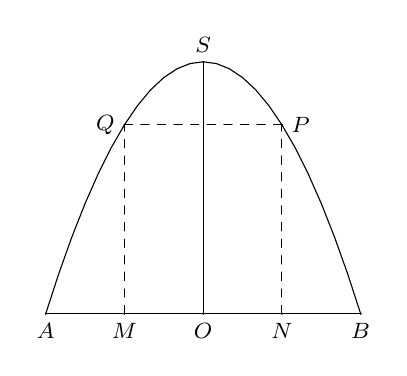
\begin{tikzpicture}[scale=.4, font=\footnotesize,line join=round, line cap=round,>=stealth,declare function={rt=.03; xmin=-5;xmax=5;ymin=0;ymax=8;}]
%\draw[color=gray!50,dashed] (\xmin,\ymin) grid (\xmax,\ymax);
\draw[-] (xmin,0)--(0,0) node[below]{$O$} --(xmax,0) node[below] {$B$};
\draw[-] (0,ymin)--(0,ymax) node[above] {$S$};
\fill (0,0) circle (1pt);
\draw[dashed] (2.5,0)--(2.5,6)node[right]{$P$} (-2.5,0)--(-2.5,6)node[left]{$Q$} (-5,0)node[below]{$A$} (-2.5,0)node[below]{$M$} (2.5,0)node[below]{$N$};
\draw[black] plot[domain=-5:5](\x,{-0.32*(\x)^2+8});
\draw[dashed] (2.5,6)--(-2.5,6);
\fill (-5,0) circle (1pt);
\fill (5,0) circle (1pt);
\fill (-2.5,0) circle (1pt);
\fill (2.5,0) circle (1pt);
\fill (2.5,6) circle (1pt);
\fill (-2.5,6) circle (1pt);
\fill (0,8) circle (1pt);
\end{tikzpicture}
}
\shortans[]{$30$}
\loigiai{
\begin{center}
\begin{tikzpicture}[scale=.5, font=\footnotesize,line join=round, line cap=round,>=stealth,declare function={xmin=-5;xmax=5;ymin=0;ymax=8;}]
\draw [->] (-6.4,0)--(6.5,0) node [below] {$x$};
\draw [->] (0,-1.5)--(0,9.5) node [left] {$y$};
\draw[-] (xmin,0)--(0,0) node[below left]{$O$} --(xmax,0) node[below] {$B$};
\draw[-] (0,ymin)--(0,ymax) node[above right] {$S$};
\fill (0,0) circle (1pt);
\draw[dashed] (2.5,0)--(2.5,6)node[right]{$P$} (-2.5,0)--(-2.5,6)node[left]{$Q$} (-5,0)node[below]{$A$} (-2.5,0)node[below]{$M$} (2.5,0)node[below]{$N$};
\draw plot[domain=-5:5](\x,{-0.32*(\x)^2+8});
\draw[dashed] (2.5,6)--(-2.5,6);
\fill (-5,0) circle (1pt);
\fill (5,0) circle (1pt);
\fill (-2.5,0) circle (1pt);
\fill (2.5,0) circle (1pt);
\fill (2.5,6) circle (1pt);
\fill (-2.5,6) circle (1pt);
\fill (0,8) circle (1pt);
\end{tikzpicture}
\end{center}
Xét parabol $(P)\colon y=a x^2+b x+c$ $(a\ne 0)$.\\
Gọi $O$ là gốc tọa độ khi đó $AB$, $MN$ nhận $SO$ là đường trung trực.\\
Do vậy $OB=OA=5$\,m hay $B(5;0)$, $A(-5;0)$ và $SO=8$\,m hay $S(0;8)$, $ON=2{,}5$\,m hay $N(2{,}5;0)$. \\
Ta có
\[\heva{
&B(5;0)\in (P)\\
&S(0;8)\in (P)\\
&A(-5;0)\in (P)}
\Leftrightarrow\heva{
&25a+5b+c=0&\quad(1)\\
&c=8&\quad(2)\\
&25a-5b+c=0.&\quad(3)}\]
Thế $(2)$ vào $(1)$ và $(3)$ ta được
\[\heva{&25a+5b=-8\\&25a-5b=-8}
\Leftrightarrow\heva{
&a=-\dfrac{8}{25}\\&b=0.}\]
Vậy parabol $(P)\colon y=-\dfrac{8}{25}x^2+8$.\\
Xét $P(2{,}5;y)\in (P)\Rightarrow y=6$ hay $NP=6$.\\
Vậy hình chữ nhật $MNPQ$ có hai kích thước $5$, $6$ nên diện tích bằng $30$\,m$^2$.
}
\end{ex}

\begin{ex}%[0D3V2-6]%[tex hóa đề ck2-form 2025-đợt 2-Hồ Đức Bân]
Khi nuôi cá thí nghiệm trong hồ, một nhà sinh học tìm được quy luật rằng: Nếu trên mỗi đơn vị diện tích của mặt hồ có $n$ con cá thì trung bình mỗi con cá sau một vụ cân nặng $P(n)=360-10n$ (đơn vị khối lượng). Hỏi người nuôi phải thả bao nhiêu con cá trên một đơn vị diện tích để trọng lượng cá sau mỗi vụ thu được là nhiều nhất?
\shortans[0]{$3240$}
\loigiai{
Tổng trọng lượng cá thu được sau một vụ là $T(n)=n(360-10n)=360n-10 n^2$.\\
Đây là một tam thức bậc hai với ẩn là $n$ có hệ số $a=-10<0$ và $b=360$ $\Rightarrow$ $\dfrac{-b}{2a}=\dfrac{-360}{2\cdot (-10)}=18$.\\
Khi đó, $T(18)=3240$.\\
Vậy người nuôi cần thả $18$ con cá trên một đơn vị diện tích để đạt tổng trọng lượng cá lớn nhất là $3240$ (đơn vị khối lượng).
}
\end{ex}

\begin{ex}%[0-HK1-CT-4-THTHDHSG-HCM-2324]%[VN-MT-6, VM026]%[0D3V2-6]
Nhân dịp Tết sắp đến, một cửa hàng bán đồ lưu niệm dự định thiết kế hàng loạt các sản phẩm bằng kính dày $5$ mm có khắc hình cành mai lên bề mặt như \textit{Hình 1}. Trước khi đi vào sản xuất, cửa hàng đã dự trù chi phí dựa trên việc tính toán diện tích một mặt $S$ của mỗi tấm kính theo công thức như \textit{Hình 2}. Biết rằng viền của tấm kính là một phần đồ thị của hàm số bậc hai như \textit{Hình 3}. Tính chi phí kính tối thiểu để làm một sản phẩm biết mỗi mét vuông kính dày $5$ mm có giá $22\,000$ đồng, bỏ qua sự hao hụt trong quá trình cắt kính (làm tròn kết quả đến hàng đơn vị).
\begin{center}
\definecolor{green(pigment)}{rgb}{0.0, 0.65, 0.31}
\definecolor{canaryyellow}{rgb}{1.0, 0.94, 0.0}
\definecolor{gold}{rgb}{1.0, 0.84, 0.0}
\definecolor{cadmiumred}{rgb}{0.89, 0.0, 0.13}
\definecolor{brown(traditional)}{rgb}{0.59, 0.29, 0.0}
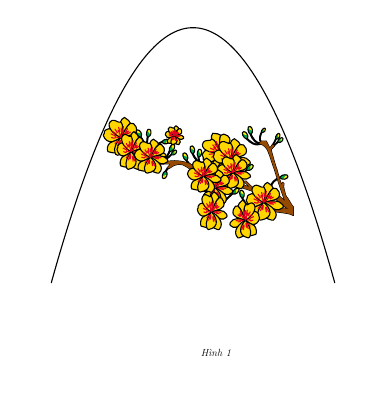
\begin{tikzpicture}[line join=round, line cap=round, >=stealth,scale=0.15, transform shape]
\clip (-14,-17) rectangle (14,12);
\tikzset{than/.pic={
\def\Canh{
(8.5,-3.2)
..controls +(140:.2) and +(-40:.2) ..(7.9,-2.3)
..controls +(150:.1) and +(-60:.1) ..(7.68,-1.58)
..controls +(130:.1) and +(-80:.1) ..(7.7,-1.2)--(7.6,-1.1)--(7.5,-1.3)
..controls +(130:.1) and +(-80:.1) ..(7.1,0)
..controls +(130:.1) and +(-80:.1) ..(6.6,1.7)--(6.9,2)--(6.75,2.1)--(6.5,1.8)--(6.2,2.4)
..controls +(140:.2) and +(-40:.2) ..(5.8,2.4)--(5.6,2.2)
..controls +(-10:.2) and +(120:.2) ..(6.2,1.8)
..controls +(-30:.2) and +(120:.2) ..(6.9,0)
..controls +(-80:.2) and +(120:.2) ..(7.8,-2.7)
..controls +(140:.2) and +(-50:.2) ..(6.6,-1.6)--(6.4,-1.6)--(6.6,-1.85)
..controls +(160:.2) and +(-30:.2) ..(5,-1.5)--(4.5,-1)--(4.3,-1)--(4.8,-1.5)
..controls +(160:.2) and +(-40:.5) ..(0,.3)
..controls +(140:.6) and +(10:.5) ..(-2,.7)
..controls +(-170:.6) and +(10:.5) ..(-4,.5)--(-4,.3)
..controls +(10:.6) and +(160:.2) ..(-1.9,.45)--(-2.2,.1)--(-2,.1)
..controls +(40:.6) and +(140:.6) ..(-.5,.2)
..controls +(-40:1) and +(155:.8) ..(7,-2.5)
..controls +(-40:.4) and +(155:.4) ..(8.2,-3.4)
..controls +(150:.4) and +(-40:.2) ..(7,-3.2)--(6.8,-3.5)
..controls +(-30:.4) and +(150:.6) ..(8.5,-3.9)--cycle

;
}
\draw[black]\Canh;
\fill[brown(traditional)] \Canh;
}}

\tikzset{bup1/.pic={
\def\B1{
(5.2,1.8)
..controls +(-155:.1) and +(-50:.1) ..(4.6,2.6)
..controls +(60:.3) and +(0:.2) ..(4.3,3.2)
..controls +(-180:.3) and +(180:.2) ..(4.5,2.6)
..controls +(-50:.5) and +(140:.1) ..(5,1.8)--cycle

;
}
\fill[green(pigment)] \B1;

\def\b1{
(4.62,2.9)
..controls +(65:.1) and +(0:.1) ..(4.3,3.2)
..controls +(-180:.2) and +(180:.5) ..cycle
;
}
\fill[canaryyellow] \b1;
\draw[black]\B1;
}}

\tikzset{bup/.pic={
\def\B{
(5.6,2.2)
..controls +(-155:.4) and +(-40:.4) ..(4.6,2.6)
..controls +(60:.3) and +(0:.2) ..(4.3,3.2)
..controls +(-180:.3) and +(180:.2) ..(4.5,2.6)
..controls +(-50:.5) and +(-155:.3) ..(5.6,2.1)
..controls +(25:.1) and +(-155:.1) ..(5.9,2.2)--cycle
;
}
\fill[green(pigment)] \B;

\def\b{
(4.62,2.9)
..controls +(65:.1) and +(0:.1) ..(4.3,3.2)
..controls +(-180:.2) and +(180:.5) ..cycle
;
}
\fill[canaryyellow] \b;
\draw[black]\B;
}}

\tikzset{mai/.pic={
\def\D{
(-6.8,2.7)
..controls +(80:.2) and +(-160:.7) ..(-6.5,4.4)
..controls +(-30:.1) and +(150:.1) ..(-6.3,4.25)
..controls +(0:.1) and +(120:.2) ..(-6,3.9)
..controls +(-150:.4) and +(50:.2) ..cycle
(-6.8,2.7)
..controls +(20:.5) and +(120:.5) ..(-5.2,2.5)
..controls +(-60:.3) and +(30:.3) ..(-5.5,2.1)
..controls +(-150:.05) and +(30:.05) ..(-5.65,2.1)
..controls +(-150:.05) and +(30:.05) ..(-5.8,2.1)
..controls +(160:.8) and +(-35:.5) ..cycle
(-6.8,2.7)
..controls +(-150:.4) and +(10:.2) ..(-7.5,2.35)
..controls +(-170:.4) and +(-75:.4) ..(-8.3,2.9)
..controls +(40:.1) and +(-85:.1) ..(-8.2,3.2)
..controls +(95:.1) and +(175:.1) ..(-7.8,3.45)
..controls +(-5:.4) and +(145:.4) ..cycle
;
}
\fill[gold] \D;
\draw[black]\D;
\def\C{

(-6,3.9)
..controls +(-150:.4) and +(50:.2) ..(-6.8,2.7)
..controls +(20:.6) and +(-70:.8) ..(-5.52,3.6)
..controls +(95:.05) and +(-30:.05) ..(-5.6,3.7)
..controls +(95:.2) and +(0:.2) ..cycle

(-6.8,2.7)
..controls +(-20:.6) and +(40:.9) ..(-6,1.2)
..controls +(-140:.1) and +(-10:.1) ..(-6.7,1.4)
..controls +(170:.1) and +(-40:.1) ..cycle

(-6.8,2.7)
..controls +(-90:.6) and +(20:.6) ..(-7.3,1.4)
..controls +(-160:.1) and +(-10:.1) ..(-7.9,1.5)
..controls +(130:.1) and +(-80:.1) ..(-7.95,1.65)
..controls +(100:.2) and +(-170:.4) ..(-7.5,2.35)
..controls +(10:.2) and +(-150:.4) ..cycle

(-6.8,2.7)
..controls +(160:.8) and +(-155:.7) ..(-7.55,4.15)
..controls +(-15:.3) and +(155:.7) ..(-7,4)
..controls +(30:.1) and +(150:.1) ..(-6.8,4)
..controls +(-30:.3) and +(80:.3) ..cycle
;
}

\fill[gold] \C;
\draw[black]\C;

\def\T{
(-6.8,2.7)
..controls +(-40:.65) and +(10:1.3) ..(-7.1,1.2)
..controls +(-170:.1) and +(-110:.05) ..(-7.3,1.4)
..controls +(120:.4) and +(-140:.4) ..cycle
;
}
\fill[gold] \T;
\draw[black]\T;
%============
\def\V{
(-6.8,2.7)
..controls +(30:.1) and +(-130:.1) ..(-6.7,2.9)
(-6.8,2.7)
..controls +(30:.1) and +(-130:.1) ..(-6.8,3)
(-6.8,2.7)
..controls +(120:.1) and +(-30:.1) ..(-6.9,2.94)
(-6.8,2.7)
..controls +(150:.1) and +(-40:.1) ..(-6.9,2.85)
;
}
\draw[cadmiumred]\V;
%\fill[ecru!80] \V;
%=================
\def\N{
(-7.3,3.4)
..controls +(-40:.05) and +(140:.05) ..(-7.1,3.1)
(-7.05,3.3)
..controls +(-40:.05) and +(120:.05) ..(-6.9,3)
(-7,3.55)
..controls +(-40:.05) and +(120:.05) ..(-6.9,3.2)
(-6.8,3.5)
..controls +(-40:.05) and +(120:.05) ..(-6.75,3.2)
(-6.6,3.3)
..controls +(-40:.05) and +(100:.05) ..(-6.7,3)
(-6.6,3.65)
..controls +(-40:.05) and +(100:.05) ..(-6.65,3.3)
(-6.3,3.25)
..controls +(-40:.05) and +(100:.05) ..(-6.5,3)
(-6.25,3.45)
..controls +(-40:.05) and +(100:.05) ..(-6.4,3.2)
(-6.35,3.05)
..controls +(40:.05) and +(-150:.05) ..(-6.15,3.25)
(-6.25,3)
..controls +(40:.05) and +(-150:.05) ..(-6,3.15)
(-6.3,2.6)
..controls +(40:.05) and +(-150:.05) ..(-6,2.55)
(-7.3,2.75)
..controls +(40:.05) and +(-150:.05) ..(-7,2.7)
(-7.6,2.7)
..controls +(-40:.05) and +(-150:.05) ..(-7.3,2.65)
(-7.65,3)
..controls +(10:.05) and +(-150:.05) ..(-7.25,2.85)
(-7.5,3.2)
..controls +(10:.05) and +(-150:.05) ..(-7.2,3)
(-7.3,2.2)
..controls +(10:.05) and +(-150:.05) ..(-7.1,2.4)
(-7.1,2)
..controls +(10:.05) and +(-150:.05) ..(-6.9,2.45)
(-6.9,2.1)
..controls +(10:.05) and +(-150:.05) ..(-6.85,2.45)
(-6.6,1.9)
..controls +(10:.05) and +(-150:.05) ..(-6.65,2.3)
(-6.4,1.9)
..controls +(10:.05) and +(-150:.05) ..(-6.58,2.3)
(-6.2,2.75)
..controls +(-150:.05) and +(20:.05) ..(-6.5,2.65)
(-6.2,2.7)
..controls +(30:.05) and +(120:.05) ..(-5.8,2.65)
(-6.65,2.8)
..controls +(30:.05) and +(-100:.05) ..(-6.5,2.95)
;
}
\draw[cadmiumred]\N;
}}

\path
(0,0)pic[scale=1]{bup}
(3.4,4.7)pic[scale=.8,rotate=-60]{bup1}
(4.5,5.55)pic[scale=.8,rotate=-80]{bup1}
(-.3,2.1)pic[scale=1,rotate=-20]{bup}
(3,5.5)pic[scale=.7,rotate=-70]{bup}
(-4.7,2)pic[scale=1,rotate=-40]{bup}
(-5.5,-1)pic[scale=1,rotate=-10]{bup}
(-5.2,.45)pic[scale=1,rotate=-20]{bup}
(-7.25,1.62)pic[yscale=-1,scale=1,rotate=-10]{bup}
(-6.5,4.2)pic[scale=1,rotate=-60]{bup1}
(-9,3.7)pic[scale=1,rotate=-40]{bup1}
(-9,.15)pic[scale=1]{bup1}
(0,2)pic[scale=1,rotate=-80]{bup1}
(1.2,4)pic[scale=1,rotate=-80]{bup1}
(-1,-3.3)pic[scale=1,rotate=-20]{bup}
(-3.5,7.5)pic[scale=1,rotate=-110]{bup}
(6.5,4.5)pic[scale=1,rotate=-110]{bup}
(-4.5,4.5)pic[scale=.8,rotate=-80]{bup1}
;
\path (0,0)pic[scale=1]{than}
(0.7,0)pic[scale=1]{mai}
(1.8,1.5)pic[scale=.5]{mai}
(.2,-1.2)pic[xscale=.8]{mai}
(0.3,0)pic[scale=0.5]{mai}
(2.5,-1.4)pic[scale=.9]{mai}
(9.5,2.5)pic[scale=1,rotate=30]{mai}
(10,-1.8)pic[scale=1]{mai}
(9.5,-2.7)pic[scale=.9]{mai}
(8,-4)pic[scale=.9]{mai}
(7,-3)pic[scale=.9]{mai}
(7,-6.3)pic[xscale=.8]{mai}
(12.8,-5.5)pic[scale=1]{mai}
(-1,-7)pic[xscale=-.8,rotate=0]{mai}
;
\draw[smooth,samples=100,domain=-12:12] plot(\x,{-.15*(\x)^2+12});
%		 \draw (2,-12) node[above] {$Hình 1$};
\draw (2,-16) node[above] {\fontsize{80}{80}\selectfont \textit{Hình 1}};
\end{tikzpicture}
\begin{tikzpicture}[>=stealth,x=1cm,y=1cm,scale=0.8]
\def\xmin{-4}\def\xmax{4}\def\ymin{0}\def\ymax{6}
\draw[<->] (2,0)--(2,4) node[midway, right] {\footnotesize $h$};
\draw[<->] (0,0)--(4,0) node[midway, below] {\footnotesize $d$};
\clip (-1.2,-1.5)rectangle(6.2,5.5);
\draw[smooth,samples=200,domain=0:4] plot (\x,{-1*((\x)^2)+4*(\x)});
\draw (2,5.5) node[below] {$S=\dfrac{2}{3}hd$};
\draw (2,-1.5) node[above] {\textit{Hình 2}};
\end{tikzpicture}
\begin{tikzpicture}[>=stealth,x=1cm,y=1cm,scale=0.8]
\def\a{-1}
\def\d{4}
\def\b{-0.5}
\def\c{1}
\draw[->] (-1,0)--(5.5,0)node[below]{$x\left(\text{mm}\right)$};
\draw[->] (0,-1)--(0,5)node[right]{$y\left(\text{mm}\right)$};
\draw (0,0)node[below right]{\footnotesize $O$};
\clip (-1.2,-1.5)rectangle(6.5,5.5);
\draw[thick,samples=150,smooth,domain=0:4] plot(\x,{\a*(\x)^2+\d*(\x)});
\draw [dashed] (2,0)--(2,4)--(0,4);
\draw (1.85,4.3) node[right]{$A$};
\draw (4,0) node[above right]{$B$};
\draw (2.6,3) node[above right]{$y=-\dfrac{1}{25}x^2+4x$};
\foreach \x/\y in {0/0,0/4,2/4,4/0}{\fill (\x,\y) circle (1pt);}
\draw (2,-0.7) node[below] {\textit{Hình 3}};
\end{tikzpicture}
\end{center}
\shortans[]{$1\,467$}
\loigiai{
Phương trình $-\dfrac{1}{25}x^2+4x=0\Leftrightarrow\hoac{&x=0\\&x=100}$ nên tọa độ điểm $B\left(100;0\right)$, tức $d=100$ (mm).\\
Tọa độ đỉnh của parabol là $A\left(50;100\right)$ nên $h=100$ (mm).\\
Vậy diện tích của mỗi tấm kính là $\dfrac{2}{3}\cdot100\cdot100=\dfrac{20\,000}{3}$ mm$^2=\dfrac{1}{150}\,\left(\text{m}^2\right)$.\\
Chi phí sản xuất một tấm kính là $\dfrac{1}{150}\cdot22\,0000\approx1\,467$ đồng.
}
\end{ex}

\begin{ex}%[0D3V2-6]%[Dự án đề kiểm tra Toán 10 CHKII NH23-24- Ngô Tất Thành]%[THPT Chuyên Hùng Vương - Tỉnh Phú Thọ]
Một cánh cổng hình bán nguyệt rộng $8{,}4$ m và cao $4{,}2$ m. Mặt đường dưới cổng được chia làm hai làn đều nhau cho xe ra vào. Một chiếc xe tải rộng $2{,}8$ m không chở hàng nếu đi đúng làn đường quy định và có thể đi qua cổng mà không làm hư cổng thì chiều cao của xe không vượt quá bao nhiêu mét (làm tròn đến hàng phần trăm)?
\begin{center}
\begin{tikzpicture}[scale=0.7,line join=round,line cap=round,font=\footnotesize,>=stealth]
\def\xmin{-4.3} \def\xmax{4.3}
\def\ymin{0} \def\ymax{5}
\definecolor{capri}{rgb}{0.0, 0.75, 1.0}
\definecolor{orange(colorwheel)}{rgb}{1.0, 0.5, 0.0}
\definecolor{kellygreen}{rgb}{0.3, 0.73, 0.09}
\fill[color=capri] (-5,2)--(-5,5)--(5,5)--(5,2);
\fill[color=gray!40!white] (-3.5,0)--(-3.5,3.05)--(3.5,3.05)--(3.5,0);

\def\Q{  (3.5,3)..controls +(120:1) and +(60:1) .. (-3.5,3);}

\draw[color=white, line width=5] \Q;

\fill[color=kellygreen] (-5,-1.5)--(-5,2)--(5,2)--(5,-1.5);
\fill[color=orange(colorwheel)] (-5,0)--(-5,3)--(5,3)--(5,0);
\pattern[pattern color=white, pattern=bricks] (-5,0)--(-5,3)--(5,3)--(5,0);

\fill[gray!50!white] (3.5,0)--(3.5,3)..controls +(120:1) and +(60:1) .. (-3.5,3)--(-3.5,0)--cycle;
\fill[white] (1,4.5)..controls +(120:.8) and +(30:1) .. (2.5,4.4)
..controls +(80:.5) and +(120:1) .. (4.8,4.3)
..controls +(-60:1) and +(-120:.6) .. (3.5,4)
..controls +(-60:.7) and +(-120:.6) .. (2,4.1)
..controls +(-60:.6) and +(-120:.6) .. (-1,4.3)
..controls +(60:.4) and +(30:.2)  .. (1,4.5);
\draw[color=white, line width=2.5] (-5,3)--(-3.5,3)--(-3.5,0) (3.5,0)--(3.5,3)--(5,3);
\fill[color=gray!80!white, line width=2] (3,0) arc (0:180:3 cm and 3cm)--cycle;
\draw[color=cyan, line width=2] (3,0) arc (0:180:3 cm and 3cm)--cycle;
\fill[color=kellygreen, line width=2,yshift=.4cm] (2.5,0) arc (0:180:2.5 cm and 2.5cm)--cycle;
\draw[color=gray, line width=2,yshift=.4cm] (2.5,0) arc (0:180:2.5 cm and 2.5cm)--cycle;
\fill[color=capri, line width=2,yshift=1.93cm] (1.914,0) arc (40:140:2.5 cm and 2.6cm)--cycle;
\fill[color=white] (-.6,2)--(-5.4,-2)--(5.4,-2)--(.6,2)--cycle;
\fill[color=gray!80!white] (-.4,2)--(-4.2,-1.5)--(4.2,-1.5)--(.4,2)--cycle;
\fill[color=white](-.2,-1.1)--(.2,-1.1)--(.3,-1.5)--(-.3,-1.5)--cycle (-.15,.7)--(.15,.7)--(.25,0)--(-.25,0)--cycle (-.1,2)--(.1,2)--(.2,1.5)--(-.2,1.5)--cycle;
\draw[color=red, line width=1.5,->] (0,0)--(3,0);
\draw[color=red, line width=1.5,->] (0,0)--(-3,0);
\node[color=red] at (0,-.5){$8{,}4$ m};
\node[color=red] at (0,1.2){$4{,}2$ m};
\draw[color=cyan, line width=1.5,->] (0,0.9)--(0,0);
\draw[color=cyan, line width=1.5,->] (0,1.5)--(0,3);
\end{tikzpicture}
\end{center}
\shortans{$2{,}33$}
\loigiai{
Ghép hệ trục tọa độ $Oxy$ vào cổng hình bán nguyệt sao cho trục $Ox$ nằm trên mặt đường, trục $Oy$ thẳng lên đỉnh của cổng, gốc tọa độ $O$ trùng với trung điểm của hai chân cổng.\\
Khi đó $A(-4{,}2;0)$, $B(4{,}2;0)$ và $C(0;4{,}2)$ thuộc mép cổng.\\
Gọi Parabol $y=ax^2+bx+c,\, a \ne 0$ là đường cong của cổng.\\
Khi đó ta có hệ phương trình
$\heva{
&a(-4{,}2)^2+b(-4{,}2)+c=0\\
&a(4{,}2)^2+b(4{,}2)+c=0}
\Leftrightarrow \heva{
&a=-\dfrac{5}{21}\\
&b=0.}$\\
Khi đó Parabol có dạng $y=-\dfrac{5}{21}x^2+4{,}2$.\\
Xe tải rộng $2{,}8$ m khi đó ta có\\
$y=-\dfrac{5}{21}(2{,}8)^2+4{,}2=\dfrac{7}{3} \approx 2{,}33$.\\
Vậy chiều cao của xe tải không quá $2{,}33$ m.
}
\end{ex}

\begin{ex}%[0D3V2-6]
Một quả bóng được đá lên từ độ cao $1{,}5$ mét so với mặt đất. Biết quỹ đạo của quả bóng là một đường parabol trong mặt phẳng toạ độ $Oxy$ có phương trình $h=at^{2} +bt+c\; \left(a<0\right)$ trong đó $t$ là thời gian (tính bằng giây) kể từ khi quả bóng được đá lên và $h$ là độ cao (tính bằng mét) của quả bóng. Biết rằng sau $2$ giây thì nó đạt độ cao $5$ m; sau $4$ giây nó đạt độ cao $4{,}5$ m. Hỏi sau $5{,}5$ giây quả bóng đạt độ cao bao nhiêu mét so với mặt đất?
\shortans[0]{$1{,}5$}
\loigiai{
Theo giả thiết ta có hệ phương trình sau \\
$\heva{h\left(0\right)&=\dfrac{3}{2} \\ h\left(2\right)&=5 \\ h\left(4\right)&=\dfrac{9}{2}} \Leftrightarrow \heva{a\left(0\right)^{2} +b\left(0\right)+c& =\dfrac{3}{2} \\ a\left(2\right)^{2} +b\left(2\right)+c&=5 \\ a\left(4\right)^{2} +b\left(4\right)+c&=\dfrac{9}{2}} \Leftrightarrow \heva{c&=\dfrac{3}{2} \\ 4a+2b+c&=5 \\ 16a+4b+c&=\dfrac{9}{2}} \Leftrightarrow \heva{a&=-\dfrac{1}{2} \\ b&=\dfrac{11}{4} \\ c&=\dfrac{3}{2}} $.\\
Suy ra $h=-\dfrac{1}{2} t^{2} +\dfrac{11}{4} t+\dfrac{3}{2}$. Khi $t=5,5$ suy ra $h=1{,}5$.\\
Vậy sau $5{,}5$ giây thì quả bóng đạt độ cao $1{,}5$ mét so với mặt đất.
}
\end{ex}

\begin{ex}%[Đề ôn tập số 02-Tổng hiệu hai véc-tơ]%[Nguyễn Trung Kiên, dự án BG10]%[0H5H2-4]
Cho tam giác $ABC$ có $AB=5$, $AC=5\sqrt{3}$ và $\widehat{BAC}=150^\circ$. Tính độ dài của véc-tơ $\overrightarrow{AC}-\overrightarrow{AB}$ (kết quả làm tròn đến hàng phần mười).
\shortans{13,2}
\loigiai{
Ta có $\left|\overrightarrow{AC}-\overrightarrow{AB}\right|=\left|\overrightarrow{BC}\right|=BC$.\\
Tam giác $ABC$ có $AB=5$, $AC=5\sqrt{3}$ và $\widehat{BAC}=60^\circ$ nên \[BC^2=AB^2+AC^2-2AB\cdot AC \cdot \cos{A}=25+75-2\cdot 5\cdot 5\sqrt{3} \cdot \cos{150^\circ}=175.\]
Vậy $\left|\overrightarrow{AC}-\overrightarrow{AB}\right| =BC=5\sqrt{7} \approx 13{,}2$.\\
}
\end{ex}

\begin{ex}%[0H5H2-4]
Cho hình vuông $ABCD$ có cạnh là $3$. Tính $\left|2\overrightarrow{AD}+\overrightarrow{AB}\right|$. (Kết quả ghi dưới dạng số thập phân và làm tròn đến hàng phần chục)
\shortans[]{$6{,}7$}
\loigiai{
\begin{center}
\begin{tikzpicture}[scale=0.8, font=\footnotesize,line join=round, line cap=round, >=stealth]
\def\canh{3}
\coordinate (A) at (0,0);
\coordinate (D) at (\canh,0);
\coordinate (B) at (0,\canh);
\coordinate (C) at ($(B)+(D)-(A)$);
\coordinate (M) at (2*\canh,0);
\coordinate (N) at (2*\canh,\canh);
\draw (B)--(N)--(M) (C)--(D);
\draw[->] (A)--(D);
\draw[->] (A)--(M);
\draw[->] (A)--(B);
\foreach \i/\g in {A/-90,B/90,C/90,D/-90,M/-90,N/90}{\draw[fill=black](\i) circle (1pt) ($(\i)+(\g:3mm)$) node[scale=1]{$\i$};}
\end{tikzpicture}
\end{center}
Dựng $\overrightarrow{AM}=2\overrightarrow{AD}$ và hình chữ nhật $ABNM$.\\
$\left| 2\overrightarrow{AD}+\overrightarrow{AB}\right|=\left| \overrightarrow{AM}+\overrightarrow{AB}\right|=\left| \overrightarrow{AN}\right|=AN=\sqrt{3^2+6^2}=3\sqrt{5}$.\\
Vậy $\left| 2\overrightarrow{AD}+\overrightarrow{AB}\right|=3\sqrt{5}\approx 6{,}7$.
}
\end{ex}

\begin{ex}%[Đề ôn tập số 02-Tổng hiệu hai véc-tơ]%[Nguyễn Trung Kiên, dự án BG10]%[0H5H2-4]
Cho tam giác $ABC$ cân tại $A$, có $AB= 6 \mathrm{\, cm}$, $\widehat{BAC}= 120^\circ$. Gọi $M$ là trung điểm của cạnh $BC$. Độ dài của véc-tơ $\overrightarrow{AB}- \overrightarrow{CM}$ bằng bao nhiêu $\mathrm{cm}$?
\shortans{3}
\loigiai
{
\begin{center}
\begin{tikzpicture}[>=stealth,line join=round,line cap=round,font=\footnotesize,scale=1]
\path
(0,0) coordinate (A)
($(A)+(-150:3)$) coordinate (B)
($(A)+(-30:3)$) coordinate (C)
($(B)!.5!(C)$) coordinate (M)
;
\draw (A)--(B)--(C)--(A)--(M);
\draw[fill=black]
(A) circle (1pt) node[above] {$A$}
(B) circle (1pt) node[below] {$B$}
(C) circle (1pt) node[below] {$C$}
(M) circle (1pt) node[below] {$M$}
;
\end{tikzpicture}
\end{center}
Vì tam giác $ABC$ cân tại $A$, $\widehat{BAC}=120^\circ$ nên tam giác $ABM$ vuông tại $M$ và $\widehat{ABM}= 30^\circ$.\\
Do đó $AM= AB \sin \widehat{ABM}= 6 \sin 30^\circ = 3 \mathrm{\, cm}$.\\
Ta có $M$ là trung điểm của $BC$ nên $\overrightarrow{MC}=\overrightarrow{BM}$. Suy ra
\[\left| \overrightarrow{AB}- \overrightarrow{CM}\right|= \left| \overrightarrow{AB}+ \overrightarrow{MC}\right|= \left| \overrightarrow{AB}+ \overrightarrow{BM}\right| = \left| \overrightarrow{AM}\right|= AM= 3\, \mathrm{cm}.\]
}
\end{ex}

\begin{ex}%[Đề ôn tập số 02-Tổng hiệu hai véc-tơ]%[Nguyễn Trung Kiên, dự án BG10]%[0H5H2-4]
Cho hình vuông $ABCD$ có cạnh bằng $\sqrt{5}$. Tính $\left|\overrightarrow{BA}+\overrightarrow{BC}-\overrightarrow{DA} \right|$ (kết quả làm tròn đến hàng phần trăm).
\shortans{3,16}
\loigiai{
\immini
{Vì $ABCD$ là hình vuông có cạnh bằng $\sqrt{5}$ nên $BD=\sqrt{5}\cdot \sqrt{2} = \sqrt{10}$.\\
Ta có $\overrightarrow{BC}=\overrightarrow{AD}=-\overrightarrow{DA}$, $\overrightarrow{BA}+\overrightarrow{BC} =\overrightarrow{BD}$.\\
Vậy $\left|\overrightarrow{BA}-\overrightarrow{DA}\right| =\left|\overrightarrow{BA}+\overrightarrow{BC}\right| =\left|\overrightarrow{BD}\right| = BD =\sqrt{10} \approx 3{,}16$.}
{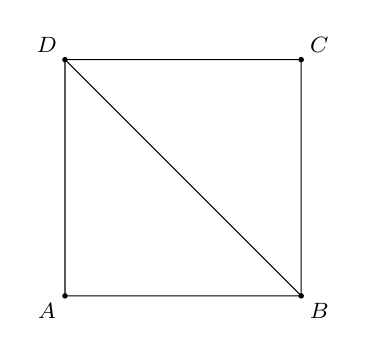
\begin{tikzpicture}[font=\footnotesize, line join=round, line cap=round, >=stealth, scale=1]
\path (0,0)coordinate (A)--(0:3) coordinate (B)--++(90:3)coordinate (C)--++(180:3)coordinate (D);
\draw (A)--(B)--(C)--(D)--(A) (B)--(D);
\foreach \y/\g in {A/220,B/-40,C/40,D/140} \fill (\y) circle (1pt)+(\g:0.3)node {$\y$};
\end{tikzpicture}}
}
\end{ex}

\begin{ex}%[0H5H2-4]
Cho $\Delta ABC$ vuông tại $A$ và $AB=1$, $AC=2$. Biết $\left|\overrightarrow{MA}\right|=\sqrt a $ và $M$ thỏa $\overrightarrow{AC}-\overrightarrow{AB}=\overrightarrow{AM}$. Giá trị của $a$ bằng
\shortans{$5$}
\loigiai{
Ta có: $\left|\overrightarrow{MA}\right|=\left|\overrightarrow{AM}\right|=\left|\overrightarrow{AC}-\overrightarrow{AB}\right|=\left|\overrightarrow{BC}\right|=BC=\sqrt{2^2+1^2}=\sqrt 5 $.
}
\end{ex}
